\documentclass[onesided]{article}\usepackage[]{graphicx}\usepackage[]{color}
% maxwidth is the original width if it is less than linewidth
% otherwise use linewidth (to make sure the graphics do not exceed the margin)
\makeatletter
\def\maxwidth{ %
  \ifdim\Gin@nat@width>\linewidth
    \linewidth
  \else
    \Gin@nat@width
  \fi
}
\makeatother

\definecolor{fgcolor}{rgb}{0.345, 0.345, 0.345}
\newcommand{\hlnum}[1]{\textcolor[rgb]{0.686,0.059,0.569}{#1}}%
\newcommand{\hlstr}[1]{\textcolor[rgb]{0.192,0.494,0.8}{#1}}%
\newcommand{\hlcom}[1]{\textcolor[rgb]{0.678,0.584,0.686}{\textit{#1}}}%
\newcommand{\hlopt}[1]{\textcolor[rgb]{0,0,0}{#1}}%
\newcommand{\hlstd}[1]{\textcolor[rgb]{0.345,0.345,0.345}{#1}}%
\newcommand{\hlkwa}[1]{\textcolor[rgb]{0.161,0.373,0.58}{\textbf{#1}}}%
\newcommand{\hlkwb}[1]{\textcolor[rgb]{0.69,0.353,0.396}{#1}}%
\newcommand{\hlkwc}[1]{\textcolor[rgb]{0.333,0.667,0.333}{#1}}%
\newcommand{\hlkwd}[1]{\textcolor[rgb]{0.737,0.353,0.396}{\textbf{#1}}}%
\let\hlipl\hlkwb

\usepackage{framed}
\makeatletter
\newenvironment{kframe}{%
 \def\at@end@of@kframe{}%
 \ifinner\ifhmode%
  \def\at@end@of@kframe{\end{minipage}}%
  \begin{minipage}{\columnwidth}%
 \fi\fi%
 \def\FrameCommand##1{\hskip\@totalleftmargin \hskip-\fboxsep
 \colorbox{shadecolor}{##1}\hskip-\fboxsep
     % There is no \\@totalrightmargin, so:
     \hskip-\linewidth \hskip-\@totalleftmargin \hskip\columnwidth}%
 \MakeFramed {\advance\hsize-\width
   \@totalleftmargin\z@ \linewidth\hsize
   \@setminipage}}%
 {\par\unskip\endMakeFramed%
 \at@end@of@kframe}
\makeatother

\definecolor{shadecolor}{rgb}{.97, .97, .97}
\definecolor{messagecolor}{rgb}{0, 0, 0}
\definecolor{warningcolor}{rgb}{1, 0, 1}
\definecolor{errorcolor}{rgb}{1, 0, 0}
\newenvironment{knitrout}{}{} % an empty environment to be redefined in TeX

\usepackage{alltt}
\usepackage[T1]{fontenc}
\linespread{1.5} % Line spacing - Palatino needs more space between lines
\usepackage{microtype} % Slightly tweak font spacing for aesthetics

\usepackage[hmarginratio=1:1,columnsep=20pt]{geometry} % Document margins
%\usepackage{multicol} % Used for the two-column layout of the document
\usepackage[hang, small,labelfont=bf,up,textfont=it,up]{caption} % Custom captions under/above floats in tables or figures
\usepackage{booktabs} % Horizontal rules in tables
\usepackage{float} % Required for tables and figures in the multi-column environment - they need to be placed in specific locations with the [H] (e.g. \begin{table}[H])

\usepackage{lettrine} % The lettrine is the first enlarged letter at the beginning of the text
\usepackage{paralist} % Used for the compactitem environment which makes bullet points with less space between them

% to ignore texts: good for thank messages and paper submissions.
      % \fbox{\phantom{This text will be invisible too, but a box will be printed arround it.}}

\usepackage{abstract} % Allows abstract customization
\renewcommand{\abstractnamefont}{\normalfont\bfseries} % Set the "Abstract" text to bold
%\renewcommand{\abstracttextfont}{\normalfont\small\itshape} % Set the abstract itself to small italic text

\usepackage[]{titlesec} % Allows customization of titles
\renewcommand\thesection{\Roman{section}} % Roman numerals for the sections
\renewcommand\thesubsection{\Roman{subsection}} % Roman numerals for subsections
\titleformat{\section}[block]{\large\scshape\centering}{\thesection.}{1em}{} % Change the look of the section titles
\titleformat{\subsection}[block]{\large}{\thesubsection.}{1em}{} % Change the look of the section titles

\usepackage{fancybox, fancyvrb, calc}
\usepackage[svgnames]{xcolor}
\usepackage{physics}
\usepackage{epigraph}
\usepackage{longtable}
\usepackage{pdflscape}
\usepackage{graphics}
\usepackage{pbox} % \pbox{20cm}{This is the first \\ cell}
\usepackage{amsfonts}
\usepackage{amsmath}
\usepackage{amssymb}
\usepackage{rotating}
\usepackage{paracol}
\usepackage{textcomp}
\usepackage[export]{adjustbox}
\usepackage{afterpage}
\usepackage{filecontents}
\usepackage{color}
\usepackage{latexsym}
\usepackage{lscape}       %\begin{landscape} and \end{landscape}
\usepackage{wasysym}
\usepackage{dashrule}
\usepackage{marvosym} % face package
\usepackage{framed}
\usepackage{tree-dvips}
\usepackage{pgffor}
\usepackage[]{authblk}
\usepackage{setspace}
\usepackage{array}
\usepackage[latin1]{inputenc}
\usepackage{hyperref}     %desactivar para link rojos
\usepackage{graphicx}
\usepackage{dcolumn} % for R tables
\usepackage{multirow} % For multirow in tables
\usepackage{pifont}
\usepackage{listings}
\usepackage{bm}




% hypothesis / theorem package begin
\usepackage{amsthm}
\usepackage{thmtools}
\declaretheoremstyle[
spaceabove=6pt, spacebelow=6pt,
headfont=\normalfont\bfseries,
notefont=\mdseries, notebraces={(}{)},
bodyfont=\normalfont,
postheadspace=0.6em,
headpunct=:
]{mystyle}
\declaretheorem[style=mystyle, name=Hypothesis, preheadhook={\renewcommand{\thehyp}{H\textsubscript{\arabic{hyp}}}}]{hyp}

\usepackage{cleveref}
\crefname{hyp}{hypothesis}{hypotheses}
\Crefname{hyp}{Hypothesis}{Hypotheses}
% hypothesis / theorem package end


%----------------------------------------------------------------------------------------
% Other ADDS-ON
%----------------------------------------------------------------------------------------

% independence symbol \independent
\newcommand\independent{\protect\mathpalette{\protect\independenT}{\perp}}
\def\independenT#1#2{\mathrel{\rlap{$#1#2$}\mkern2mu{#1#2}}}







\hypersetup{
    bookmarks=true,         % show bookmarks bar?
    unicode=false,          % non-Latin characters in Acrobat's bookmarks
    pdftoolbar=true,        % show Acrobat's toolbar?
    pdfmenubar=true,        % show Acrobat's menu?
    pdffitwindow=true,     % window fit to page when opened
    pdfstartview={FitH},    % fits the width of the page to the window
    pdftitle={My title},    % title
    pdfauthor={Author},     % author
    pdfsubject={Subject},   % subject of the document
    pdfcreator={Creator},   % creator of the document
    pdfproducer={Producer}, % producer of the document
    pdfkeywords={keyword1} {key2} {key3}, % list of keywords
    pdfnewwindow=true,      % links in new window
    colorlinks=true,       % false: boxed links; true: colored links
    linkcolor=ForestGreen,          % color of internal links (change box color with linkbordercolor)
    citecolor=ForestGreen,        % color of links to bibliography
    filecolor=ForestGreen,      % color of file links
    urlcolor=ForestGreen           % color of external links
}

%\usepackage[nodayofweek,level]{datetime} % to have date within text

\newcommand{\LETT}[3][]{\lettrine[lines=4,loversize=.2,#1]{\smash{#2}}{#3}} % letrine customization



% comments on margin
  % Select what to do with todonotes: 
  % \usepackage[disable]{todonotes} % notes not showed
  \usepackage[draft]{todonotes}   % notes showed
  % usage: \todo{This is a note at margin}

\usepackage{cooltooltips}

%%% bib begin
\usepackage[american]{babel}
\usepackage{csquotes}
\usepackage[backend=biber,style=authoryear,dashed=false,doi=false,isbn=false,url=false,arxiv=false]{biblatex}
%\DeclareLanguageMapping{american}{american-apa}
\addbibresource{/Users/hectorbahamonde/Bibliografia_PoliSci/library.bib} 
\addbibresource{/Users/hectorbahamonde/Bibliografia_PoliSci/Bahamonde_BibTex2013.bib} 

% USAGES
%% use \textcite to cite normal
%% \parencite to cite in parentheses
%% \footcite to cite in footnote
%% the default can be modified in autocite=FOO, footnote, for ex. 
%%% bib end

\usepackage{fancyhdr} % Headers and footers
\pagestyle{fancy} % All pages have headers and footers
\fancyhead{} % Blank out the default header
\fancyfoot{} % Blank out the default footer
\fancyhead[C]{MLE para Outcomes Censurados/Truncados: Tobit Models} % Custom header text
\fancyfoot[RO,LE]{\thepage} % Custom footer text
\IfFileExists{upquote.sty}{\usepackage{upquote}}{}
\begin{document}
% DOCUMENT ID
%----------------------------------------------------------------------------------------
%	CONTENT
%----------------------------------------------------------------------------------------

%\graphicspath{
%{/Users/hectorbahamonde/RU/Term5/Experiments_Redlawsk/Experiment/Data/}
%}



%%%%%%%%%%%%%%%%%%%%%%%%%%%%%%%%%%%%%%%%%%%%%%
% begin knitr stuff


%%%%%%%%%%%%%%%%%%%%%%%%%%%%%%%%%%%%%%%%%%%%%%





\hspace{-5mm}{\bf Profesor}: H\'ector Bahamonde, PhD.\\
\texttt{e:}\href{mailto:hector.bahamonde@uoh.cl}{\texttt{hector.bahamonde@uoh.cl}}\\
\texttt{w:}\href{http://www.hectorbahamonde.com}{\texttt{www.hectorbahamonde.com}}\\
{\bf Curso}: MLE.\\
\hspace{-5mm}{\bf TA}: Gonzalo Barr\'ia.

\section{Outcomes Censurados/Truncados}

En esta clase pensaremos en la variables dependientes truncadas o censuradas $y_{\star}$. \emph{Censored} es diferente a \emph{truncated}. Como veremos en esta clase,

\begin{enumerate}
  \item {\bf Censuradas}: Las variables dependientes censuradas $y^{\star}_{i}$ son aquellas donde a pesar de observar todo el dataset, s\'olo tenemos informaci\'on parcial de $y_{i}$.
  \item {\bf Truncadas}: Las variables dependientes truncadas $y^{\star}_{i}$ son aquellas donde (por alg\'un motivo) no vemos todo el dataset, y en consecuencia s\'olo tenemos informaci\'on parcial de $y_{i}$.
\end{enumerate}

Tambi\'en es posible ver las diferencias conceptuales entre variables truncadas y censuradas de manera gr\'afica:

{\centering 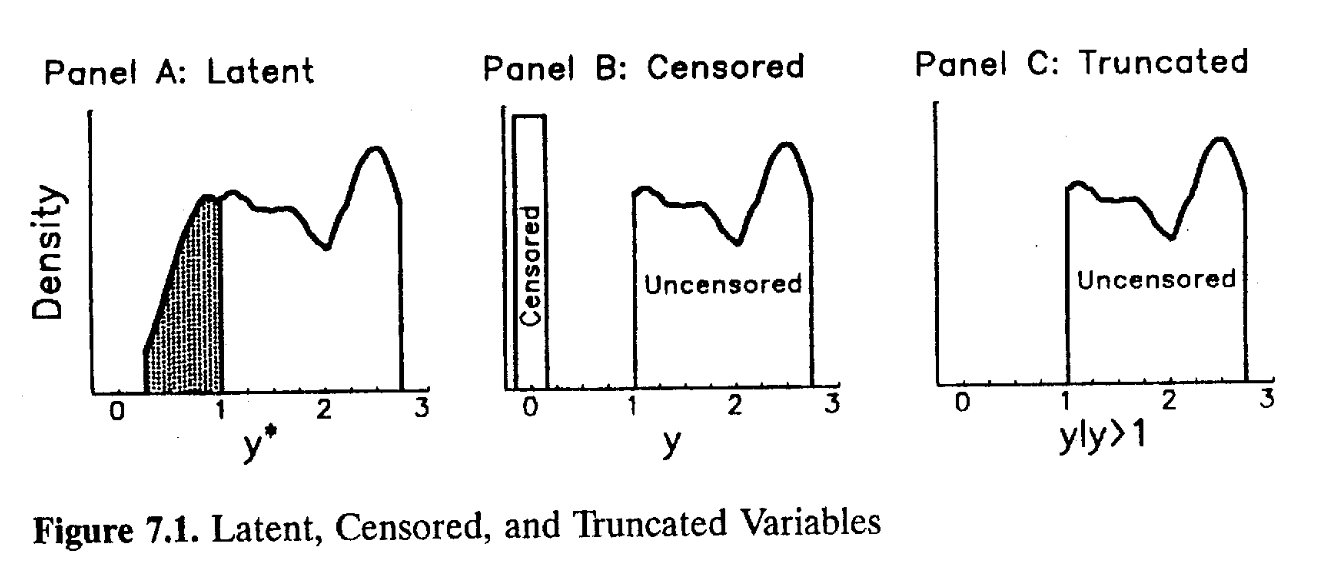
\includegraphics[width=\maxwidth]{fig_7_1.png}}


Afortunadamente tenemos los modelos \texttt{tobit} para estimarlos. Como veremos, ambos procesos (\emph{censored}/\emph{truncated}) asumen supuestos distribucionales diferentes.

{\centering 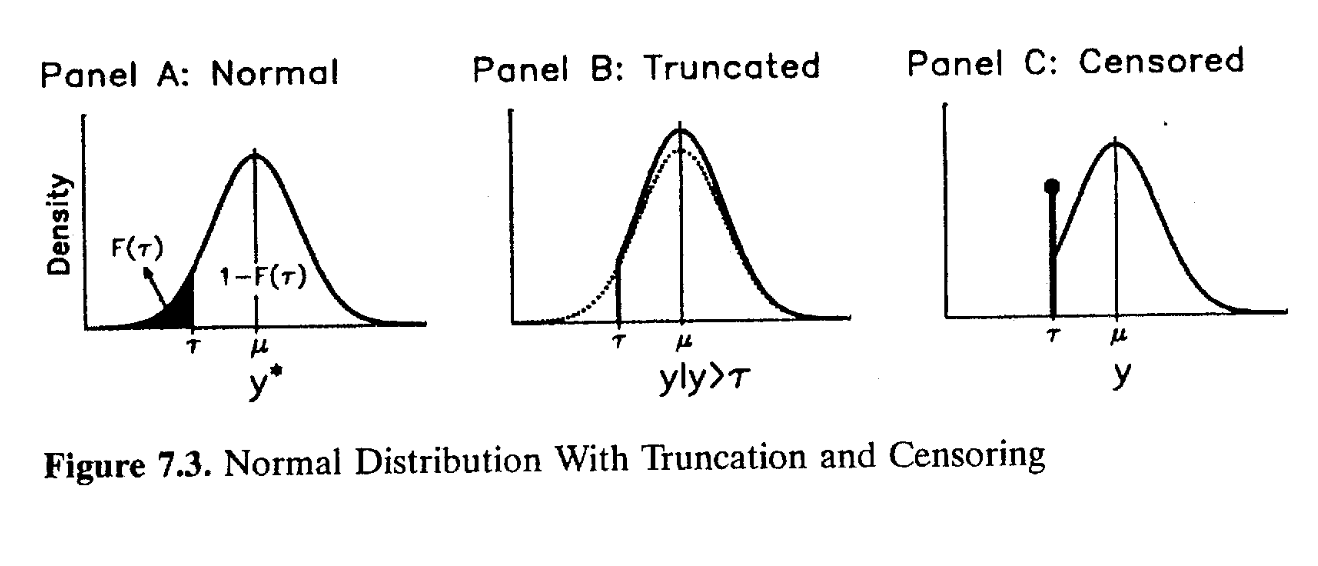
\includegraphics[width=\maxwidth]{fig_7_3.png}}

Como ves en la Figura 7.3, las distribuciones de $y^{\star}_{i}$ var\'ian seg\'un el tipo de ignorancia con el que estamos lidiando. {\bf Nota que uno de los supuestos de la especificaci\'on del modelo \texttt{tobit} es que $y^{\star}_{i}$ est\'a normalmente distribuido}.



\subsection{Censored Data}

Las variables dependientes censuradas $y^{\star}_{i}$ son aquellas donde a pesar de observar todo el dataset, s\'olo tenemos informaci\'on parcial de $y_{i}$. El t\'ipico ejemplo es cuando en las encuestas preguntan por los ingresos, y las escalas est\'an truncadas: \emph{Menos de \$100} (1) o \emph{M\'as de \$1.000} (10). En el primer caso, respondentes que ganan \$25 ser\'an codificados como ``1'' al igual que alguien que gana \$95. Esto se llama \emph{left-censoring}. A la derecha (\emph{right-censoring}) ser\'ia el caso de alguien que gane \$1.500: ella ser\'a codificada como ``10'' al igual que alguien que gane \$999. Nota que observas todo el dataset: es s\'olo que la estructura de la variable ``censura'' cierta informaci\'on, convirtiendo $y_{i}$ en $y_{i}^{\star}$.

Continuaremos motivando el modelo \texttt{tobit} v\'ia modelos latentes. Existe una variable no censurada o truncada $y_{i}$ que no podemos observar. En vez, observamos la variable censurada $y^{\star}_{i}$, donde,

\[
    y_{i}= 
\begin{cases}\label{censored:1}
    y_{i}^{\star} & \text{si} \; y_{i}^{\star} > 1 \\
    0           & \text{si} \; y_{i}^{\star} \leq 1
\end{cases}
\]

En este ejemplo seguimos la Figura 7.2 para el caso espec\'ifico de que veamos $y_{i}^{\star}$ s\'olo cuando $y_{i}^{\star}\geq1$, pero \emph{no} veamos nada cuando $y_{i}^{\star}\leq1$. Obviamente, el umbral puede variar seg\'un la especificaci\'on.

{\centering 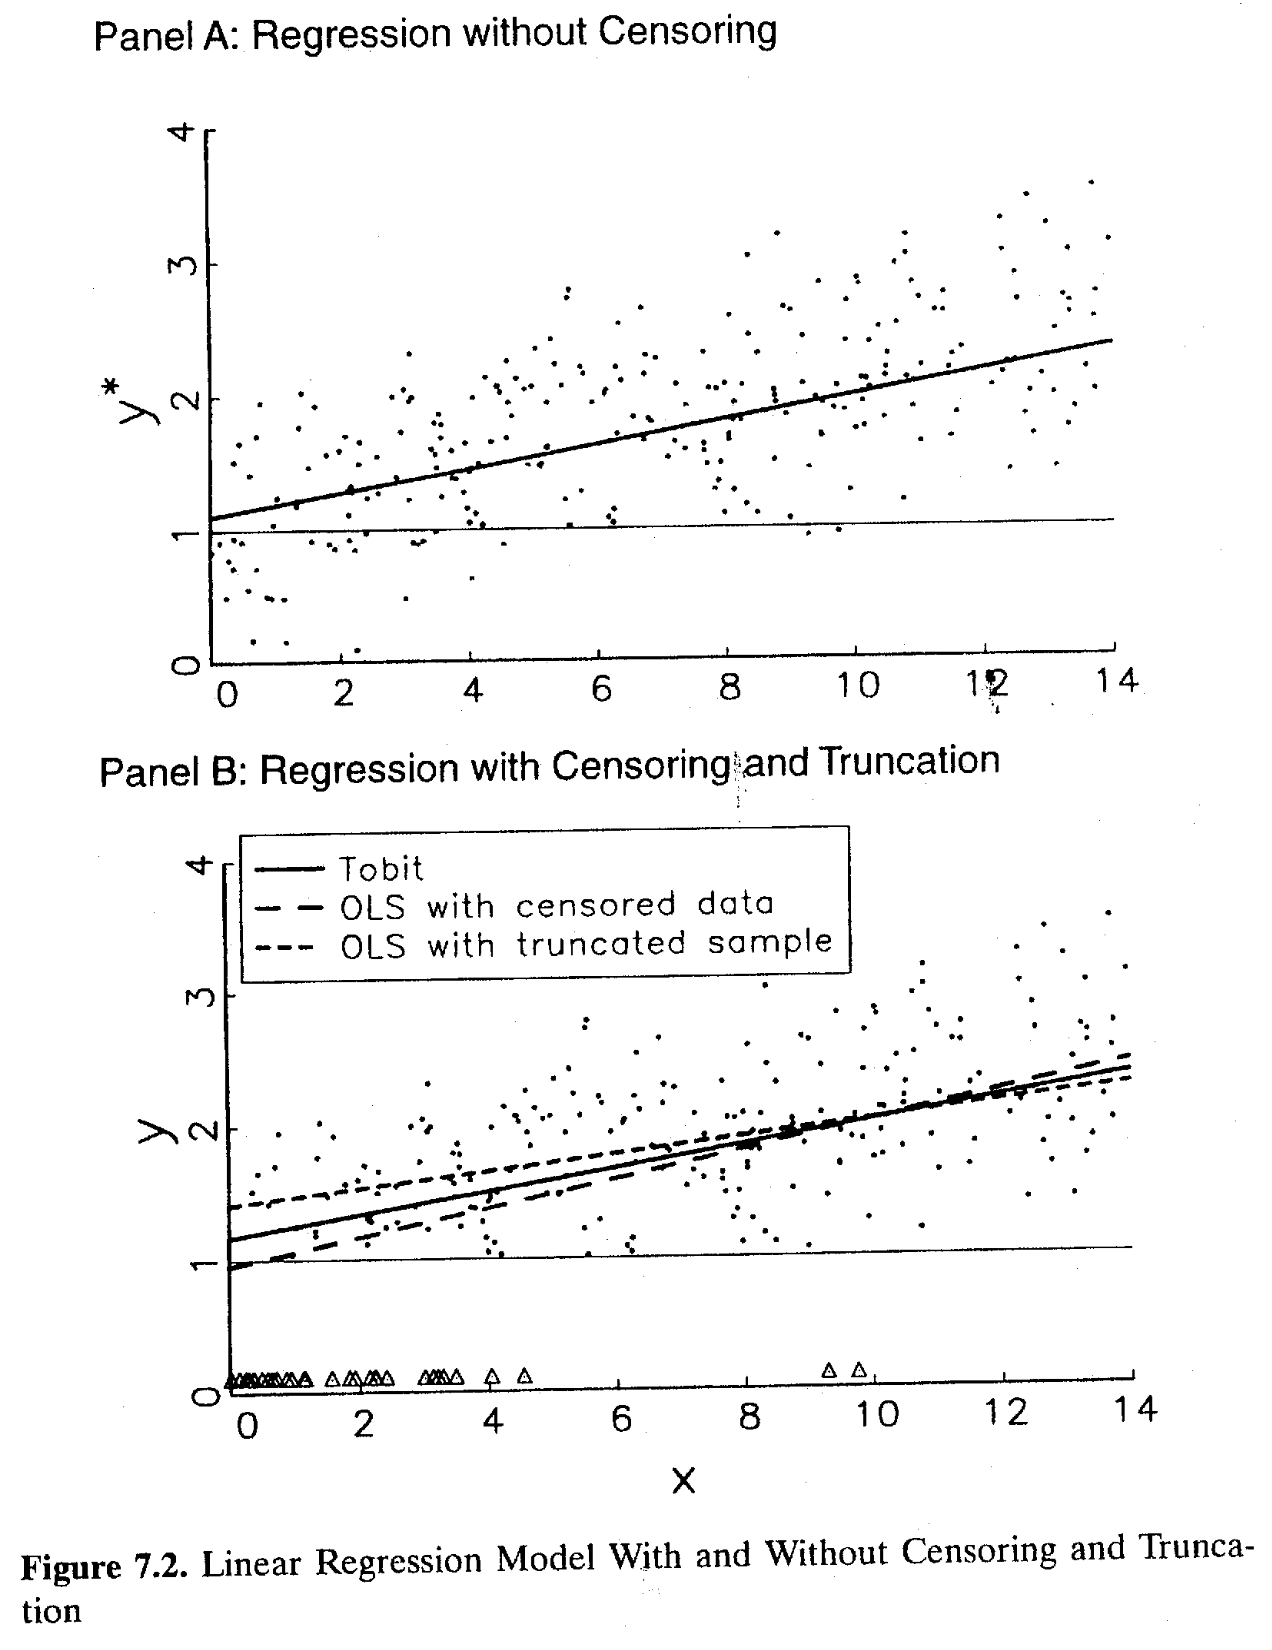
\includegraphics[width=\maxwidth]{fig_7_2.png}}


Como lo muestra \textcite[189]{Long1997}, los coeficientes $\boldsymbol{\beta}$ estar\'an mal estimados si se usan m\'etodos lineales. Para ello existe el modelo \texttt{tobit}.

\paragraph{Supuestos distribucionales} 

La distribuci\'on normal truncada:

\begin{equation}\label{censored:2}
f(y| y > \tau, \mu, \sigma) = \frac{\frac{1}{\sigma}\Phi(\frac{y_{i}^{\star}-\mu}{\sigma})}{1-\Phi(\frac{\tau-\mu}{\sigma})}
\end{equation}


donde $\Phi$ es el \emph{probability density function} de la distribuci\'on normal est\'andard, y $\tau$ es un ``threshold'' (o ``umbral'') bajo el cual se censuran valores de $y_{i}$. 

Es importante tambi\'en notar que $\Phi(\frac{\tau-\mu}{\sigma})$ en \autoref{censored:2} es la probabilidad de que $y_{i}$ est\'e censurado \parencite[195]{Long1997}. Esto implica que que la probabilidad de \emph{no} estar censurado es $1-\Phi(\frac{\tau-\mu}{\sigma})$. 

Como explica \textcite[199]{Long1997}, existe un link entre el modelo \texttt{tobit} y el \emph{probit}. Nota que no s\'olo ambos modelos estructurales son iguales, sino que tambi\'en (y tal como lo mostramos en \autoref{censored:5}), la probabilidad de que una observaci\'on sea censurada se calcula usando un modelo parecido al \emph{probit}.

\paragraph{Estimaci\'on} 


El modelo estructural \texttt{tobit} est\'a dado por algo que ya debiera ser familiar,


\begin{equation}\label{censored:3}
y_{i}^{\star} = \boldsymbol{x}_{i}\boldsymbol{\beta} + e_{i}
\end{equation}

donde $e_{i}$ es homoesqued\'astico y $e_{i}\sim N (0, \sigma^{2})$ \parencite[206]{Long1997}. Esto implica que un modelo \texttt{tobit} con \emph{right-censoring} est\'a dado por,

%\begin{equation}\label{censored:4}
\[
    y_{i}= 
\begin{cases}\label{censored:4}
    y_{i}^{\star} = \boldsymbol{x}_{i}\boldsymbol{\beta} + e_{i}  & \text{si} \; y_{i}^{\star} < 1 \\
    \tau_{y}           & \text{si} \; y_{i}^{\star} \geq \tau
\end{cases}
\]
%\end{equation}

Lo interesante de la especificaci\'on \texttt{tobit} es que modela (mediante supuestos distribucionales) la probabilidad de que un sujeto sea censurado, de manera tal que,

\begin{equation}\label{censored:5}
Pr(y_{i}^{\star} \leq \tau | \boldsymbol{x}_{i}) = Pr(\epsilon_{i} \leq \tau - \boldsymbol{x}_{i}\boldsymbol{\beta}|\boldsymbol{x}_{i}) = \Phi(\frac{\tau-\boldsymbol{x}_{i}\boldsymbol{\beta}}{\sigma})
\end{equation}

Esta informaci\'on es muy \'util. Debido a que no sabemos los valores de $y_{i}^{\star}\leq\tau$, nosotros usamos la proabilidad de ser censurado como si fuera el likelihood \parencite[204-205]{Long1997}. En otras palabras, debido a que no conocemos los valores de $y_{i}^{\star}\leq\tau$, no podemos usar el alto de la curva normal para estimar el likelihood (ver Figura 7.8). Afortunadamente, debido a que conocemos la igualdad $y_{i}^{\star}\leq\tau$, y que observamos $\boldsymbol{x}$, podemos calcular \autoref{censored:5}.


{\centering 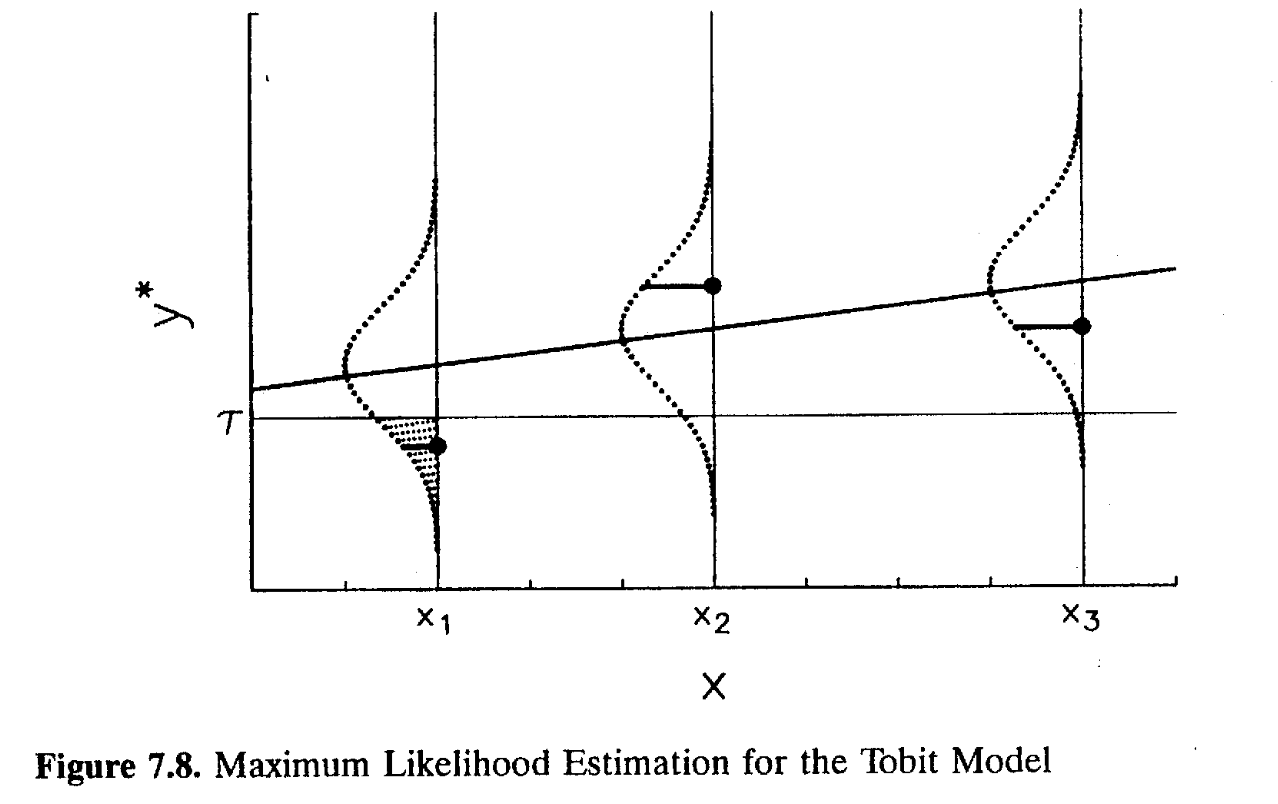
\includegraphics[width=\maxwidth]{fig_7_8.png}}

En consecuencia, la funci\'on likelihood para \emph{uncensored outcomes} (``U'') est\'a dada por,

\begin{equation}\label{censored:6}
lnL_{U}(\boldsymbol{\beta},\sigma^{2}) = \sum_{U}ln\frac{1}{\sigma}\Phi-(\frac{y_{i}-\boldsymbol{x}_{i}\boldsymbol{\beta}}{\sigma})
\end{equation}

mientras que la funci\'on likelihood para \emph{censored outcomes} (``C'') est\'a dada por,

\begin{equation}\label{censored:7}
lnL_{C}(\boldsymbol{\beta},\sigma^{2}) = \sum_{C}ln\Phi-(\frac{\tau-\boldsymbol{x}_{i}\boldsymbol{\beta}}{\sigma})
\end{equation}

\subsection{Truncated Data}

El modelo estructural de los procesos truncados es igual. Lo mismo ocurre con su likelihood. La \'unica diferencia es que el likelihood debe ser ajustado por el \'area de la distribuci\'on normal que ha sido truncada. {\bf Nota, en consecuencia, que el supuesto de la normalidad es fundamental en el modelo \texttt{tobit}}.

\section{Programaci\'on}

\textcite[811]{Greene2011} explica que la base de datos \texttt{Affairs} pregunta el n\'umero de relaciones extra maritales en un a\~no. 

Carguemos los datos:

\begin{knitrout}
\definecolor{shadecolor}{rgb}{0.969, 0.969, 0.969}\color{fgcolor}\begin{kframe}
\begin{alltt}
\hlkwd{library}\hlstd{(AER)}
\hlkwd{data}\hlstd{(}\hlstr{"Affairs"}\hlstd{)}
\end{alltt}
\end{kframe}
\end{knitrout}

Hagamos un resumen de la variable dependiente,

\begin{knitrout}
\definecolor{shadecolor}{rgb}{0.969, 0.969, 0.969}\color{fgcolor}\begin{kframe}
\begin{alltt}
\hlkwd{table}\hlstd{(Affairs}\hlopt{$}\hlstd{affairs)}
\end{alltt}
\begin{verbatim}
## 
##   0   1   2   3   7  12 
## 451  34  17  19  42  38
\end{verbatim}
\end{kframe}
\end{knitrout}

Como ves, los c\'odigos ``7'' y ``12'' est\'an censurados. El primero (``7'') significa 4-10 \emph{affairs}, y ``12'' una categor\'ia superior. 

El paquete de \texttt{R} que usaremos se llama \texttt{AER}, y la funci\'on se llama \texttt{tobit}.

\begin{knitrout}
\definecolor{shadecolor}{rgb}{0.969, 0.969, 0.969}\color{fgcolor}\begin{kframe}
\begin{alltt}
\hlstd{tobit.m} \hlkwb{<-} \hlkwd{tobit}\hlstd{(affairs} \hlopt{~} \hlstd{age} \hlopt{+} \hlstd{yearsmarried} \hlopt{+} \hlstd{religiousness} \hlopt{+} \hlstd{occupation} \hlopt{+} \hlstd{rating,}
                 \hlkwc{right} \hlstd{=} \hlnum{4}\hlstd{,}
                 \hlkwc{data} \hlstd{= Affairs)}
\end{alltt}
\end{kframe}
\end{knitrout}

F\'ijate que hemos declarado que tenemos \emph{right-censoring} desde el c\'odigo ``4''. Hagamos una tabla.

\begin{kframe}
\begin{alltt}
\hlkwd{p_load}\hlstd{(texreg)}
\hlkwd{texreg}\hlstd{(tobit.m)} \hlcom{# usa "screenreg" no "texreg".}
\end{alltt}
\end{kframe}
\begin{table}
\begin{center}
\begin{tabular}{l c}
\hline
 & Model 1 \\
\hline
(Intercept)    & $7.90^{**}$   \\
               & $(2.80)$      \\
age            & $-0.18^{*}$   \\
               & $(0.08)$      \\
yearsmarried   & $0.53^{***}$  \\
               & $(0.14)$      \\
religiousness  & $-1.62^{***}$ \\
               & $(0.42)$      \\
occupation     & $0.32$        \\
               & $(0.25)$      \\
rating         & $-2.21^{***}$ \\
               & $(0.45)$      \\
Log(scale)     & $2.07^{***}$  \\
               & $(0.11)$      \\
\hline
AIC            & $1014.09$     \\
BIC            & $1044.88$     \\
Log Likelihood & $-500.04$     \\
Deviance       & $581.31$      \\
Total          & $601$         \\
Left-censored  & $451$         \\
Uncensored     & $70$          \\
Right-censored & $80$          \\
Wald Test      & $42.56$       \\
\hline
\multicolumn{2}{l}{\scriptsize{$^{***}p<0.001$; $^{**}p<0.01$; $^{*}p<0.05$}}
\end{tabular}
\caption{Statistical models}
\label{table:coefficients}
\end{center}
\end{table}



\paragraph{Interpretaci\'on}  Debido a que nuestra variable es continua, los modelos \texttt{tobit} se pueden interpretar igual que un modelo OLS. {\bf Interpretemos la tabla}.


Estimemos las \emph{predicted probabilities},

\begin{knitrout}
\definecolor{shadecolor}{rgb}{0.969, 0.969, 0.969}\color{fgcolor}\begin{kframe}
\begin{alltt}
\hlstd{y.hat} \hlkwb{=} \hlkwd{predict}\hlstd{(tobit.m,} \hlkwc{interval} \hlstd{=} \hlstr{"prediction"}\hlstd{)}
\end{alltt}
\end{kframe}
\end{knitrout}


Ahora hagamos dos gr\'aficos, que por propositos demostrativos, s\'olo seleccionaremos dos variables.

\begin{knitrout}
\definecolor{shadecolor}{rgb}{0.969, 0.969, 0.969}\color{fgcolor}\begin{kframe}
\begin{alltt}
\hlkwd{par}\hlstd{(}\hlkwc{mfrow}\hlstd{=}\hlkwd{c}\hlstd{(}\hlnum{1}\hlstd{,}\hlnum{2}\hlstd{))}
\hlkwd{plot}\hlstd{(Affairs}\hlopt{$}\hlstd{yearsmarried, y.hat);}\hlkwd{abline}\hlstd{(}\hlkwd{lm}\hlstd{(y.hat} \hlopt{~} \hlstd{Affairs}\hlopt{$}\hlstd{yearsmarried))}
\hlkwd{plot}\hlstd{(Affairs}\hlopt{$}\hlstd{religiousness, y.hat);}\hlkwd{abline}\hlstd{(}\hlkwd{lm}\hlstd{(y.hat} \hlopt{~} \hlstd{Affairs}\hlopt{$}\hlstd{religiousness))}
\end{alltt}
\end{kframe}

{\centering 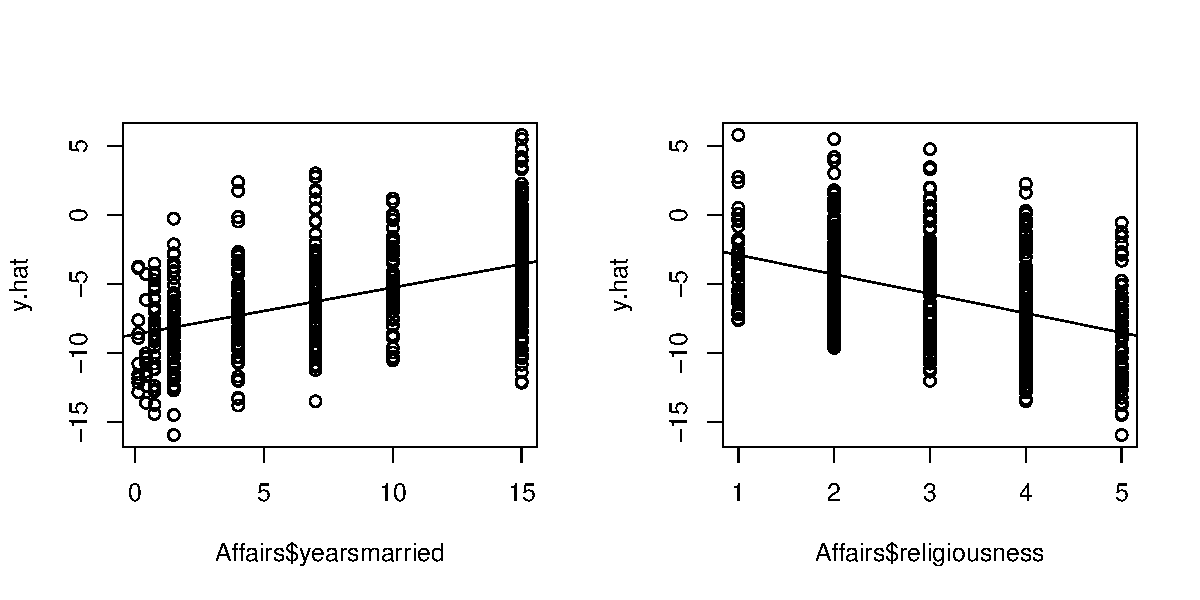
\includegraphics[width=\maxwidth]{figure/pp:plot-1} 

}



\end{knitrout}

Finalmente, hagamos un diagn\'ostico r\'apido. Veamos los residuos. Primero, hagamos el c\'alculo.

\begin{knitrout}
\definecolor{shadecolor}{rgb}{0.969, 0.969, 0.969}\color{fgcolor}\begin{kframe}
\begin{alltt}
\hlstd{e} \hlkwb{=} \hlstd{Affairs}\hlopt{$}\hlstd{affairs} \hlopt{-} \hlstd{y.hat}
\end{alltt}
\end{kframe}
\end{knitrout}

Veamos si tienen promedio cero.

\begin{knitrout}
\definecolor{shadecolor}{rgb}{0.969, 0.969, 0.969}\color{fgcolor}\begin{kframe}
\begin{alltt}
\hlkwd{mean}\hlstd{(e)}
\end{alltt}
\begin{verbatim}
## [1] 7.326525
\end{verbatim}
\end{kframe}
\end{knitrout}

Ahora veamos el gr\'afico. Siempre gr\'afica tus residuos.

\begin{knitrout}
\definecolor{shadecolor}{rgb}{0.969, 0.969, 0.969}\color{fgcolor}\begin{kframe}
\begin{alltt}
\hlkwd{plot}\hlstd{(y.hat, e)}
\hlkwd{abline}\hlstd{(}\hlkwc{h}\hlstd{=}\hlnum{0}\hlstd{,} \hlkwc{col}\hlstd{=}\hlstr{"blue"}\hlstd{)}
\end{alltt}
\end{kframe}

{\centering 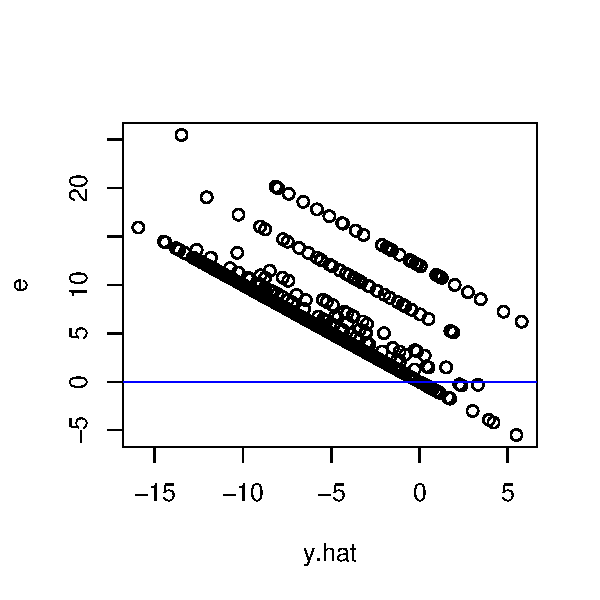
\includegraphics[width=\maxwidth]{figure/residuals:3-1} 

}



\end{knitrout}


\begin{knitrout}
\definecolor{shadecolor}{rgb}{0.969, 0.969, 0.969}\color{fgcolor}\begin{kframe}
\begin{alltt}
\hlstd{knitr}\hlopt{::}\hlkwd{purl}\hlstd{(}\hlstr{'Tobit.Rnw'}\hlstd{)}
\end{alltt}
\begin{verbatim}
## [1] "Tobit.R"
\end{verbatim}
\begin{alltt}
\hlkwd{Stangle}\hlstd{(}\hlstr{'Tobit.Rnw'}\hlstd{)}
\end{alltt}
\begin{verbatim}
## Writing to file Tobit.R
\end{verbatim}


{\ttfamily\noindent\bfseries\color{errorcolor}{\#\# Error in match.arg(options\$results, c("{}verbatim"{}, "{}tex"{}, "{}hide"{})): 'arg' should be one of "{}verbatim"{}, "{}tex"{}, "{}hide"{}}}\end{kframe}
\end{knitrout}


\newpage
\paragraph{}
\paragraph{}
\pagenumbering{Roman}
\setcounter{page}{1}
\printbibliography



\end{document}

